%!TEX encoding = UTF-8 Unicode
%!TEX program = xelatex

\documentclass[bachelor]{ustcthesis}
% bachelor|master|doctor
\usepackage{ustcextra}
\usepackage{pgfplots}
\usepackage{multirow}
\usepackage[position=top]{subfig}
\graphicspath{{figures/}}
%\bibliographystyle{ustcauthoryear}
\bibliographystyle{ustcnumerical}

\title{多线程并行 InSAR 数据处理\\程序的设计与实现}
\author{崔灏}
\major{固体地球物理专业}
\advisor{查显杰\ 副教授}
\submitdate{二〇一七年五月}
%\secrettext{机密\quad 小于等于20年}   % 内部|秘密|机密,注释本行则不保密
\depart{地球和空间科学学院}

\entitle{Design and implementation of multi-threaded parallel InSAR processing program}
\enauthor{CUI Hao}
\enmajor{Solid Geophysics}
\enadvisor{ZHA Xianjie, Assoc. Prof.}
\ensubmitdate{May, 2017}
%\ensecrettext{Confidential\quad Less than or equal to 20 years}  % Internal|Secret|Confidential

\begin{document}

\maketitle

%
% 本科论文:
%   frontmatter: 致谢、目录、中文摘要、英文摘要
%   mainmatter: 正文章节、参考文献
%   appendix: 附录
%
% 硕博论文:
%   frontmatter: 中文摘要、英文摘要、目录、符号说明
%   mainmatter: 正文、参考文献
%   appendix: 附录
%   backmatter: 致谢、发表论文
%

\frontmatter
\begin{acknowledgements}

中国科大地球和空间科学学院查显杰副教授,作为本课题指导老师,在课题实施中给予了充分的指导和帮助。其课题组的同学们也提出了很多宝贵的意见。感谢查老师和同学们的悉心指导和帮助。

实验测试是在中科院电磁空间信息重点实验室张卫明教授课题组的 Linux 计算集群上进行的。感谢张老师课题组对课题的支持。

\end{acknowledgements}

\tableofcontents
\listoffigures
\listoftables
\begin{abstract}

星载或机载 SAR 雷达图像是地球物理研究中常用的大地测量数据源。SAR/InSAR 成像数据处理量大、算法复杂度较高,对计算设备性能有很高的要求。然而,随着 CPU 并行计算能力的提升,在消费级个人工作站上进行 SAR/InSAR 数据处理已经成为可能。

本课题研究了以 GMTSAR 为代表的 InSAR 数据处理软件的性能瓶颈,对算法中时间复杂度较高的图像拼接、图像配准模块进行了 CPU 并行优化。对真实 SAR 数据的处理结果显示,对比传统串行算法,本文提出的并行算法在不降低结果精度的前提下大大提高了多核 CPU 的使用率、缩短了计算时间。

本文设计的并行算法不依赖特殊硬件,在消费级个人工作站上即可较快地完成 InSAR 数据处理,为地球物理相关科研人员提供了便利。同时,本文的思路也可以为地球物理领域的其他科学计算任务并行优化提供参考。
    
\keywords{合成孔径干涉雷达\zhspace{} 大地测量\zhspace{} 图像处理\zhspace{} 并行计算}
\end{abstract}

\begin{enabstract}
Spaceborne and airborne Synthetic Aperture Radar (SAR) imaging is a common data source of geodesy in geophysical research. SAR/InSAR imaging processes huge amount of data and is very compute-intensive, so it typically requires computers with high performance to do it. However, with the development of parallel computing hardware, it has become possible to carry out SAR/InSAR data processing on consumer-level personal workstations.

In this paper, the performance bottleneck of InSAR data processing software (GMTSAR as a example) is studied. Compute-intensive modules such as image registration and image stitching are optimized by adopting parallel algorithms in this work. Compared with traditional serial algorithms, the parallel algorithms proposed in this paper greatly improve the performance of InSAR data processing without loss of precision.

The parallel algorithms proposed in this paper does not rely on special hardwares and works well on consumer-level workstation, which benifits geophysical researchers. Besides, the idea of parallel optimization in this paper also provides a good reference for optimization of other algorithms of scientific computing.

\enkeywords{InSAR, geodesy, image processing, parallel computing}
\end{enabstract}

%\listofalgorithms  % 算法索引,如不需要,可直接注释掉本行
% \input{chapters/notation}

\mainmatter
\chapter{绪论}


\section{研究背景}

合成孔径雷达(synthetic aperture radar, SAR)是一种高分辨率的微波雷达成像技术。机载或星载 SAR 微波雷达发射相干的微波信号并观察地面回波,通过信号处理得到尺度远大于雷达口径的等效“合成孔径”。SAR 成像分辨率可以达到米级,部分机载 SAR 系统甚至可以提供 10 cm 级的地表分辨率\cite{cantalloube2006airborne}。由于其高分辨率和全天时、全天候工作的优势,SAR 成像被广泛地用于灾害预警、遥感测绘、海洋观测、环境保护等军用和民用领域。自上世纪 80 年代以来,各国陆续发射了 ERS-1/2、Envisat、ALOS 等 SAR 卫星,星载 SAR 雷达数据成为重要的大地测量数据来源。

合成孔径雷达干涉(Interferometric SAR, InSAR)是利用多幅 SAR 图像提取高程信息的拓展应用。如果利用一组 SAR 雷达观测同一块地面区域、或者同一雷达不同时间观测同一块地面区域,由于两次观测中天线与目标相对位置存在差异(由于天线位置差异或地表形变),两幅 SAR 图像之间就会存在相位差异。相位差反映了地表高程信息或者形变信息。InSAR 成像是常用的雷达测高技术,可以取得数日到数年时间尺度上厘米级的地表形变信息,被广泛地用于地震、地面沉降、固体潮等长短周期的地表形变观测。

SAR/InSAR 成像算法是一个复杂的信号处理过程。典型的 SAR 成像算法如距离多普勒算法,它包括距离向压缩(range compression)、距离向徙动校正(range migration)和方位向压缩(azimuth compressions)三个基本步骤。信号压缩通过匹配滤波实现,可以借助快速傅立叶变换算法(Fast Fourier Transform, FFT)高效完成。SAR 数据处理技术已经比较成熟,可以通过数字信号处理器高效地实现\cite{curlander2006sar}。包括日本 ALOS 在内的许多 SAR 数据源直接向终端用户提供了 SAR 成像处理后的单视复图像(single look complex,SLC)。因此,对于地球物理研究工作等终端应用,往往可以直接下载 SLC 图像进行 InSAR 成像。

InSAR 数据处理算法时间和空间复杂度比较高。在大地测量领域,InSAR 成像范围宽度可达数百公里,处理数据量十分巨大。虽然经过数十年的发展 InSAR 数据处理程序的效率已经提高了很多,但研究人员往往会在个人工作站上进行 InSAR 数据处理,仍然需要耗费较长的时间等待结果。在桌面平台上,常用的 SAR/InSAR 数据处理软件有 GMTSAR\cite{web:gmtsar}、ISCE(InSAR Scientific Computing Environment)\cite{web:isce}等。

近年来,计算机中央处理器(Central Processing Unit, CPU)主频受制于物理极限已趋于饱和,芯片厂商转而发展多核心 CPU 技术,提高 CPU 并行处理能力。多核心 CPU 可以在同一时间并行处理多个计算任务,但每个任务的计算速度仍受制于主频。近几年的消费级个人电脑往往都已经配备具有 4 到 8 个计算核心的多核心 CPU;服务器甚至可能配置多个多核心 CPU,达到数十个逻辑计算核心。利用多个 CPU 核心进行多线程并行计算,可以使总体计算能力突破主频瓶颈。

在新兴的计算机视觉、人工智能等领域,多线程并行处理已经被广泛用于加速计算程序。而以 InSAR 数据处理为代表的地球物理科学计算领域,很多经典计算程序并未进行并行优化,计算速度仍受制于 CPU 主频。为了满足大地测量中大规模 InSAR 数据处理的需求,加速桌面平台 InSAR 数据处理,本课题以 GMTSAR 开放的算法代码为基础对 InSAR 数据处理算法的部分重要模块进行了并行优化,以期在桌面多核心 CPU 平台上减少数据处理时间。

\section{现有工作}

InSAR 成像算法已经发展得非常成熟,主要包括图像配准、干涉相位合成、相位滤波和相位解缠等基本模块。加州大学圣迭戈分校(UC San Diego)和斯克里普斯海洋研究所(Scripps Institution of Oceanography)开发的 SAR/InSAR 数据处理软件 GMTSAR 是学习这些算法的重要范本。GMTSAR 仅能使用 CPU 单线程进行 InSAR 数据处理,计算效率不高。但由于其源代码完全开放,任何人都可以免费获取并自由修改,因此在地球物理学术界应用非常广泛。\cite{sandwell2011gmtsar}

目前已经有一些针对特定硬件优化 InSAR 算法的实例。\citet{shayu2014} 在多核数字信号处理器(Digital Signal Process, DSP)上实现了实时 InSAR 数据处理,并探讨了在现场可编程逻辑门阵列(Field Programmable Gate Array, FPGA)硬件上实现高效并行 InSAR 数据处理的可行性。这类多核 DSP 芯片和 FPGA 设备具有低功耗和良好的并行性,适合在嵌入式设备上使用,比如可以整合进 SAR 雷达系统。但在桌面平台,这类特殊硬件非常少见。

图形处理器(Graphics Processing Unit, GPU)是另一类具有强大并行处理能力的微处理器,并且往往具有较大的独立内存空间(显存)。\citet{reza2015accelerating} 在 NVIDIA GPU 上借助 CUDA 通用计算框架实现了高效的相位解缠算法,对比 CPU 程序取得了数十倍的性能提升,并显著降低了计算功耗。未来,基于 GPU 的通用计算有望成为高性能计算应用的主要平台。但目前 GPU 通用计算技术还在发展阶段,在科学计算领域应用并不广泛。

\section{课题内容简介}

本课题基于 GMTSAR 公开的 InSAR 数据处理算法,选取图像配准(image registration)和图像拼接(image stitching)两个计算复杂度比较高的程序模块,设计并实现了多线程并行处理算法,以期在桌面或服务器多核心 CPU 上提高 InSAR 数据处理效率。本文详细介绍了两个并行处理算法的设计方案,并简要探讨了其他 InSAR 数据处理模块的并行优化思路。

在公开的 ALOS 卫星数据上进行的测试显示,多线程并行处理算法在不降低结果精度的条件下显著提高了多核心 CPU 平台上 InSAR 数据处理的效率。本文给出了并行算法与 GMTSAR 串行算法的性能比较数据,并定性地分析了性能提升的来源。


\chapter{算法设计和优化}

\section{InSAR 成像算法简介}

\subsection{InSAR 测高原理}

讨论并行 InSAR 成像算法之前,先对基本的算法原理做一个简单回顾。

\begin{figure}[ht]
\centering
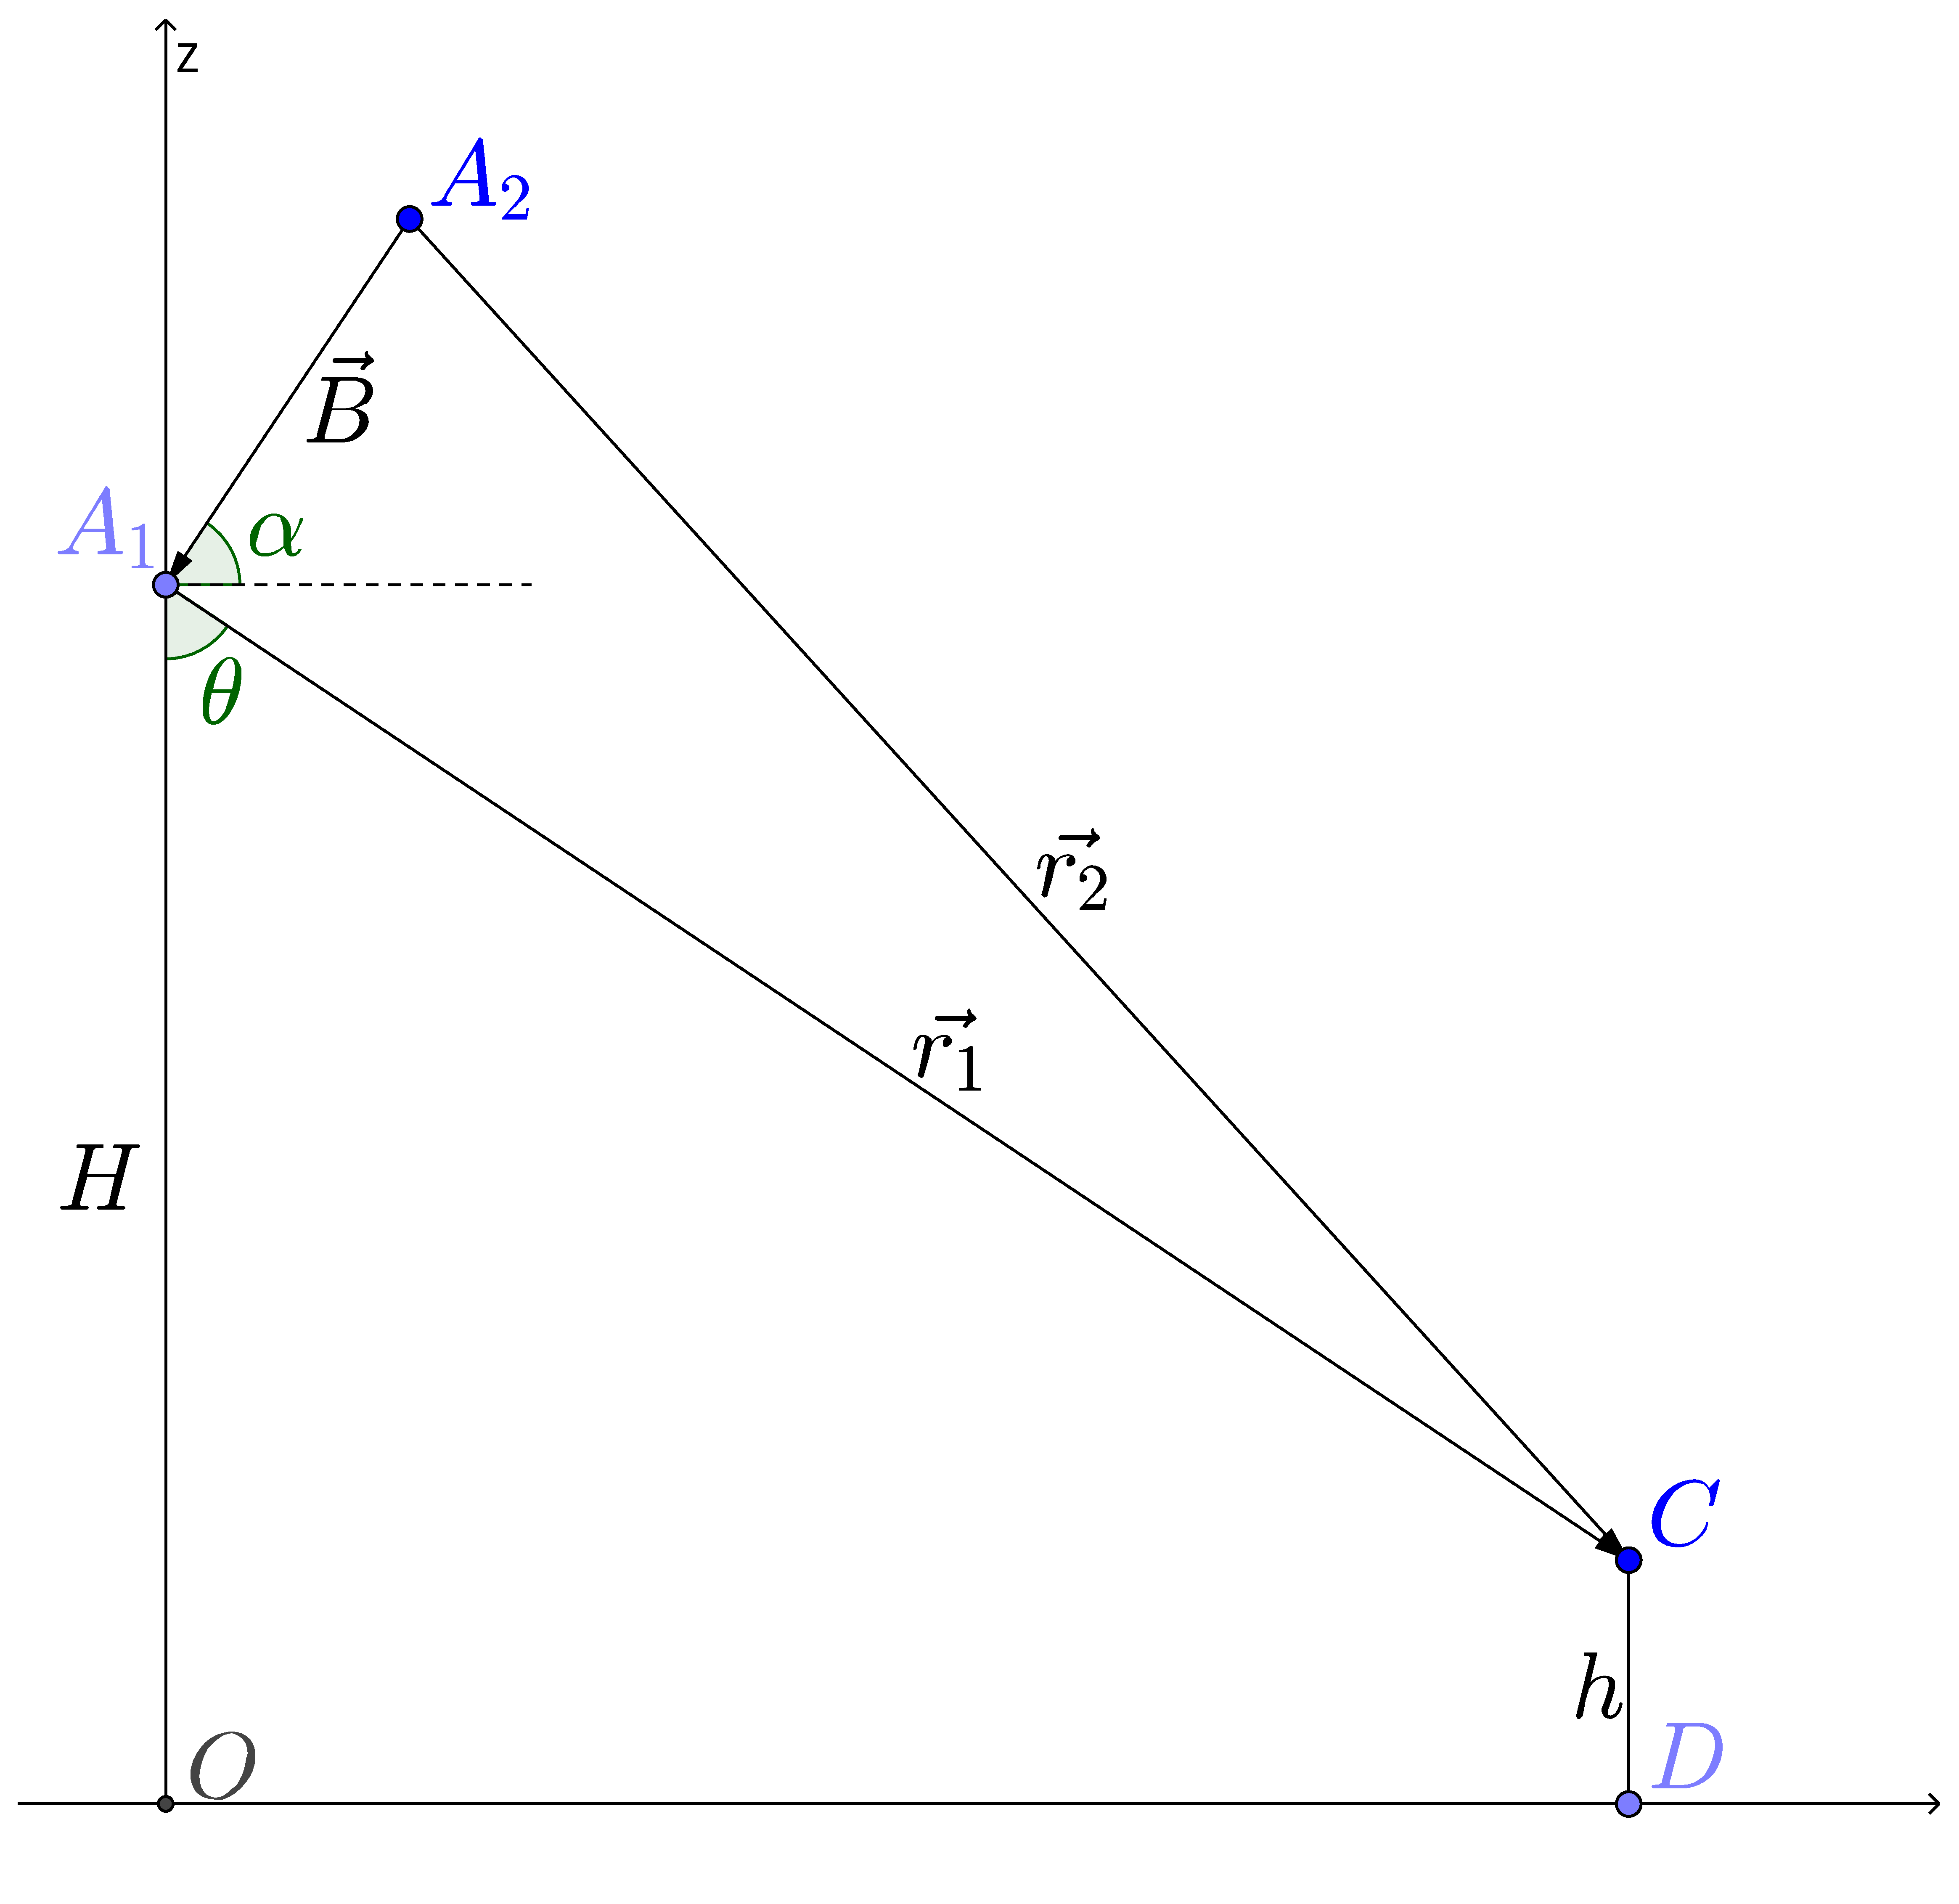
\includegraphics[width=0.4\textwidth]{insar_simple}
\caption{InSAR 高程测量基本原理} \label{fig:insar_simple}
\end{figure}

图 \ref{fig:insar_simple} 展示了利用两个 SAR 雷达观测同一地面单位进行 InSAR 测高的基本原理。InSAR 测量地表形变的原理与之类似。$A_1$ 和 $A_2$ 表示主天线和副天线位置,两天线空间位移矢量为 $\vec{B}$,称为 InSAR 基线,角度 $\alpha$ 为基线与水平面夹角。$C$ 为地面目标点,相对于两天线的位移矢量分别为 $\vec{r_1}$ 和 $\vec{r_2}$,称为斜距。角度 $\theta$ 为主天线观察方向与竖直方向的夹角,称为下视角。

斜距矢量 $ \vec{r_1} $ 和 $ \vec{r_2} $ 可以根据天线方向和微波信号双程旅行时得到;雷达位置或 SAR 卫星轨道,即基线 $\vec{B}$ 和天线高度 $H$,也可以认为是已知的。

由简单的几何关系可知,目标点高度可以表示为:

\begin{equation}
    h = H - r_1 \cos\theta
\end{equation}

为了得到 $\theta$,分别从主天线和副天线取得 SAR SLC 图像。目标点 $C$ 在两幅图像上的复像素值 $P_1$ 和 $P_2$ 可以表示为:

\begin{equation}
\begin{split}
    P_1(\vec{r_1}) = A_1(\vec{r_1}) \exp(i \frac{4\pi}{\lambda} r_1) \\
    P_2(\vec{r_2}) = A_2(\vec{r_2}) \exp(i \frac{4\pi}{\lambda} r_2) \\
\end{split}
\end{equation}

将两幅 SLC 图像共轭相乘,即得到一幅干涉图像:

\begin{equation}
    P_{\textrm{int}} = P_1^* P_2 =  A_1 A_2 \exp(i \frac{4\pi}{\lambda}(r_2 - r_1))
\end{equation}

干涉图相位项中的 $ r_2 - r_1 $ 可以通过余弦定理展开:
\begin{equation}
\begin{split}
    r_2 - r_1 &= r_1 (\frac{r_2}{r_1} - 1) \\
              &= r_1 \sqrt{1- \frac{\vec{r_1} \cdot \vec{B}}{r_1} + (\frac{B}{r_1})^2}
\end{split}
\end{equation}

基线长度 $B$ 一般远小于斜距 $r_1$、$r_2$,上式可以简化为:
\begin{equation}
    r_2 - r_1 = - \vec{r_1} \cdot \vec{B} = - r_1 B \cos(\frac{\pi}{2} - \theta + \alpha)
\end{equation}

故 $\theta$ 可以通过干涉图相位求出,进而得到目标点高程 $h$。然而,实际上回波相位(SAR 图像相位)是折叠到一个 $2\pi$ 周期内的,因此干涉图相位的值域也折叠在一个 $2\pi$ 周期中,这称为相位缠绕(phase wrap)。连续的相位值仍可以通过一些相位解缠算法估计出来。

实际使用 InSAR 测高时,还必须考虑地球曲率的影响。测量地表形变或位移时,原始地形引起的相位差也要通过数字高程模型去除。在过去,雷达轨道信息的精度也会影响 InSAR 成像精度;近些年,得益于卫星定位技术的发展,雷达轨道已经可以比较精确地获知。此外,电离层噪声、对流层噪声等因素也会影响 InSAR 成像的精度。

\subsection{InSAR 成像算法}

虽然 InSAR 测高原理非常简单,但实际的成像算法要复杂得多。主要可以归纳为以下若干步骤:

\textbf{SAR 成像和预处理}:相位差的测量精度决定了 InSAR 测高的精度。进行干涉的两幅 SAR 图像必须对成像区域有较好的聚焦,并且具有合适的基线长度,往往需要在若干组 SAR 数据中进行\textbf{筛选}。为了提取成像区域的有效信息,往往需要对 SAR 数据或者 SLC 图像进行\textbf{拼接}和\textbf{切割}。

\textbf{图像配准}:进行干涉成像之前,要通过图像配准将两幅 SAR 图像的像素精确对齐。SAR 图像像素大致对应于 SAR 雷达分辨率(数十米量级\cite{sandwell2011gmtsar})。虽然轨道数据已经可以较为精确地提供主副 SAR SLC 图像之间的偏移信息,但往往仍存在几个像素的误差。\citet{sandwell2011gmtsar} 指出,基于大地定位系统的卫星轨道数据在方位向的精度大约为1个像素、在距离向大约为2个像素。为了取得次像素级的配准精度,往往需要使用两幅图像的互相关特征进行修正。图像配准是成像程序中计算复杂度较高的一个步骤。

\textbf{干涉成像}:将对齐的主副 SAR SLC 图像进行共轭相乘,得到干涉图像。干涉图的相位被折叠到一个 $2\pi$ 周期上。根据上一节的推导,干涉图的相位信息反映了地面高程或地表位移信息。

\textbf{相位修正}:根据研究对象的不同,从干涉图中可选地去除地形相位、电离层延迟等不需要的相位项,以及滤除各种影响结果精度的噪声。

\textbf{相位解缠}:利用(一般情况下)高程或形变的连续性,从折叠相位恢复出连续变化的相位,以在较大的尺度上反映高程或形变信息。

上述步骤即为 InSAR 成像程序的主要功能。除此之外,包括 GMTSAR 在内的 InSAR 处理软件还支持地形图叠加等辅助分析功能,研究人员可以按需进一步处理。

\section{InSAR 成像算法 CPU 并行优化}

本节将以 GMTSAR 中图像拼接预处理和相位解缠两个程序模块为例子,介绍 CPU 并行的 InSAR 成像程序的算法设计和具体实现。

\subsection{并行图像配准算法设计}

GMTSAR 将主 SAR SLC 图像像素到副 SLC 图像之间的映射近似为一个二维仿射变换,可以通过6个变换参数定义。主 SLC 图像的像素 $(x_i, y_i)$ 因为轨道偏移被映射到副 SLC 图像上的 $(x_i', y_i')$,两个坐标通过仿射变换矩阵相联系:

\begin{equation}
\begin{bmatrix}
  t_i x_i' \\
  t_i y_i' \\
  t_i \\
\end{bmatrix}
= \begin{bmatrix}
       a & b & c \\
       d & e & f \\
       0 & 0 & 1 \\
\end{bmatrix}
\begin{bmatrix}
  x \\
  y \\
  1 \\
\end{bmatrix}
\end{equation}




\subsection{并行图像拼接算法设计}

\subsection{其他程序模块的并行优化}

\chapter{实验测试与分析}

本节使用的 InSAR 测试数据是 GMTSAR 官方提供的2010年4月下加利福尼亚州 $7.2 M_w$ 地震前后的 ALOS 卫星数据。主、副 SAR SLC 图像分别拍摄于2009年12月17日和2010年5月4日。SLC 图像大小为一个标准的 ALOS 图像帧,方位向和距离向长度各为 27648 像素和 11304 像素。软件测试环境如表 \ref{tab:env} 所示。

\begin{table}[htbp]
\centering
\begin{tabular}{|l|l|l|}
\hline
    \multirow{3}{*}{CPU}                        & 型号     & Intel Xeon E5-2650 v4                 \\ \cline{2-3} 
                                                & 核心数   & $\times 12$                           \\ \cline{2-3} 
                                                & 主频     & 2.20 GHz                              \\ \hline
    \multicolumn{2}{|l|}{内存}                             & 32768 MiB                             \\ \hline
    \multicolumn{2}{|l|}{操作系统}                         & Ubuntu 16.04.2 LTS, Linux 4.4.0 内核  \\ \hline
    \multicolumn{1}{|c|}{\multirow{2}{*}{编译}} & 编译器   & gcc 5.4.0                             \\ \cline{2-3} 
    \multicolumn{1}{|c|}{}                      & 编译参数 & \texttt{-O2 -march=native}            \\ \hline
\end{tabular}
\caption{软件测试环境} \label{tab:env}
\end{table}

\section{图像拼接算法测试}

并行图像拼接算法的实验测试中,因为数据来源有限,仅仅使用了6个同一轨道号的连续的 SAR 图像帧进行测试。图 \ref{fig:exp_merge} 展示了并行线程数对拼接程序性能的影响。可以看到,并行归约算法将拼接时间缩短了一半以上。比较遗憾的是,由于要拼接的图像帧数量较少,归约算法的线程数很快就收敛了,并行算法性能大概在2~3个线程时就达到了饱和。

\begin{figure}[htbp]
\centering
\subfloat[程序计算时间]{
    \label{fig:exp_merge_a}
    \begin{minipage}[t]{0.49\textwidth}
        \centering
        \resizebox {\textwidth} {!} {
            \begin{tikzpicture}
\begin{axis}[
    xlabel={并行线程数},
    ylabel={计算时间/s},
    xmin=1, xmax=7,
    ymin=0, ymax=200,
    xtick={1, 2, 3, 4, 5, 6, 7},
%    ytick={ },
    legend pos=north east,
    ymajorgrids=true,
    grid style=dashed,
]

\addplot[
    color=red,
    mark=square,
    style=solid,
    ]
    coordinates {
        (1, 194.972254756)
        (2, 106.441216719)
        (3, 91.799094679)
        (4, 92.142388643)
        (5, 92.000214744)
        (6, 88.829891908)
        (7, 83.641275544)
    };
\end{axis}
\end{tikzpicture}

        }
    \end{minipage}
}
\subfloat[CPU 核心利用率]{
    \label{fig:exp_merge_b}
    \begin{minipage}[t]{0.49\textwidth}
        \centering
        \resizebox {\textwidth} {!} {
            \begin{tikzpicture}
\begin{axis}[
    xlabel={并行线程数},
    ylabel={CPU 核心占用},
    xmin=1, xmax=7,
    ymin=0, ymax=4,
    xtick={1, 2, 3, 4, 5, 6, 7},
%    ytick={ },
    legend pos=north east,
    ymajorgrids=true,
    grid style=dashed,
]

\addplot[
    color=red,
    mark=square,
    style=solid,
    ]
    coordinates {
        (1, 1.000)
        (2, 1.862)
        (3, 2.257)
        (4, 2.258)
        (5, 2.298)
        (6, 2.425)
        (7, 2.575)
    };
\end{axis}
\end{tikzpicture}

        }
    \end{minipage}
}
\caption{线程数对 SAR 图像帧并行拼接算法性能的影响} \label{fig:exp_merge}
\note{\small 测试数据共6个 ALOS 图像帧}
\end{figure}
 
该例子说明,并行算法的性能并非总是随着线程数的增加而提升。计算线程数量超过一定值后,多余的线程将不会改善程序性能,必须改进算法或者提高数据量以增加可利用的线程数。此外,线程数量增加时,线程间通信的成本会增加,其他不可并行资源访问(如磁盘读写)也可能达到性能瓶颈。

图像拼接算法完全是确定性的,不会受拼接顺序影响。经过验证。并行拼接与顺序拼接的结果完全一致。

\section{图像配准算法测试}

图 \ref{fig:exp_cores} 展示了默认计算参数(见表 \ref{tab:xcorr-args})下 xcorr2 性能随计算线程数的变化趋势。当计算线程从无增加至6个时,图 \ref{fig:exp_cores_a} 显示的计算时间缩短非常显著。但当计算线程数进一步增加时,运行时间并没有显著变化。图 \ref{fig:exp_cores_b} 中的 CPU 核心使用率也反应了这种趋势,当计算线程数多于6个时,核心使用率少于计算线程数,说明程序已经无法充分利用所有的 CPU 核心。后面的实验中将使用8个计算线程对 xcorr2 并行性能进行评估,

\begin{figure}[htbp]
\centering
\subfloat[程序计算时间]{
    \label{fig:exp_cores_a}
    \begin{minipage}[t]{0.49\textwidth}
        \centering
        \resizebox {\textwidth} {!} {
            \begin{tikzpicture}
\begin{axis}[
    xlabel={计算线程数},
    ylabel={计算时间/s},
    xmin=0, xmax=12.2,
    ymin=0, ymax=12,
    xtick={0, 2, 4, 6, 8, 10, 12},
%    ytick={ },
    legend pos=north east,
    ymajorgrids=true,
    grid style=dashed,
]

\addplot[
    color=red,
    mark=square,
    style=solid,
    ]
    coordinates {
        (0, 11.200907922)
        (1, 10.521500231)
        (2, 5.431319614)
        (3, 3.757715043)
        (4, 2.918596810)
        (6, 2.146015373)
        (8, 2.052885075)
        (12, 2.181156634)
    };
    \legend{xcorr2} 
\end{axis}
\end{tikzpicture}

        }
    \end{minipage}
}
\subfloat[CPU 核心利用率]{
    \label{fig:exp_cores_b}
    \begin{minipage}[t]{0.49\textwidth}
        \centering
        \resizebox {\textwidth} {!} {
            \begin{tikzpicture}
\begin{axis}[
    xlabel={计算线程数},
    ylabel={占用 CPU 核心数},
    xmin=0, xmax=12.2,
    ymin=0, ymax=10,
    xtick={0, 2, 4, 6, 8, 10, 12},
%    ytick={ },
    legend pos=north west,
    ymajorgrids=true,
    grid style=dashed,
]
\addplot[
    color=red,
    mark=square,
    ]
    coordinates {
        (12,8.667)
        (8 ,7.296)
        (6 ,6.414)
        (4 ,4.438)
        (3 ,3.376)
        (2 ,2.304)
        (1 ,1.168)
        (0 ,1.000)
    };
    \legend{xcorr2}
\end{axis}
\end{tikzpicture}

        }
    \end{minipage}
}
\caption{使用不同数量计算线程对 xcorr2 配准性能的影响}
\note{xcorr2 运行时会启动一个主线程和若干计算线程,主线程不参与计算。计算线程数为0代表不启动计算线程,直接使用主线程串行计算。}
\label{fig:exp_cores}
\end{figure}

\begin{table}[htbp]
\centering
\begin{tabular}{|l|l|l|}
    \hline
    \textbf{参数} & \textbf{符号和默认值} & \textbf{对计算时间的影响(估计)} \\
    \hline
    采样位置数量         & $ n_x \times n_y = 16 \times 32 = 512 $  & $ T \propto n_x n_y $                          \\
    \hline
    采样窗口宽度         & $ w_x = w_y = 64 $                       & $ T \propto w_x w_y \log(w_x) $                \\ 
    \hline
    距离向插值因子       & $ \iota_r = 2 $                          & -                                              \\
    \hline
    互相关矩阵插值因子   & $ \iota_x = \iota_y = 16 $               & -                                              \\ 
    \hline
    计算线程数(xcorr2) & $ N_{thread} $                           & $ T \propto 1 / N_{thread} $                   \\ 
    \hline
\end{tabular}
\caption{GMTSAR xcorr / xcorr2 各项计算参数} \label{tab:xcorr-args}
\end{table}
 
接下来若干图表(图 \ref{fig:exp_nxy} 、图 \ref{fig:exp_xsys} 和图 \ref{fig:exp_ri})展示了不同配准参数对 GMTSAR xcorr 程序、串行 xcorr2 程序(即不启动计算线程,直接使用主线程计算)和多线程并行 xcorr2 程序计算性能的影响。需要注意,GMTSAR xcorr 虽然是串行算法,但由于其调用的 GMT 函数库会启动额外的线程进行其他非计算操作,因此实测的 CPU 核心占用率会略高于1。

对于评测数据涉及的三项参数对计算时间的影响,简要分析如下:

\begin{itemize}
    \item \textbf{采样窗口数量 $n_x \times n_y$}(图\ref{fig:exp_nxy})决定了局部配准算法执行的次数。局部配准算法在所有采样位置上的计算流程是完全一致的,因此理论上计算时间与采样窗口数量成正比。测试数据也印证了这一点。
    \item \textbf{采样窗口宽度 $w_x$、$w_y$}(图\ref{fig:exp_xsys})或采样窗口大小,实验中取 $w_x = w_y = w$。该参数决定了局部配准算法处理的矩阵规模。因为局部配准中的矩阵操作主要是 2D FFT 变换,故可以根据 FFT 理论估计计算时间正比于 $w^2 \log(w)$。测试数据基本上反映了这一趋势(由于 $\log(w)$ 变化较小,计算时间主要受 $w^2$ 因子影响)。
    \item \textbf{距离向插值因子 $\iota_r$}(图\ref{fig:exp_ri})对计算时间的影响并不是很容易从图中观察得出。虽然距离向插值增加了采样窗口的像素数,但实际上 xcorr 在后续计算过程仅保留了图像中心的插值点,使采样窗口仍保持 $w_x \times w_y$ 大小,因此 $\iota_r$ 影响的仅仅是与插值直接关联的一组复序列 FFT 计算。之所以单独列出,是因为注意到使用距离向插值会显著增加 xcorr 计算时间,虽然计算时间的增加并不随 $\iota_r$ 明显变化。而距离向插值对 xcorr2 计算时间的影响并不十分明显。
\end{itemize}

将 GMTSAR xcorr 与 xcorr2 配准性能横向比较,xcorr2 的性能提升十分显著,部分结果性能提升甚至达到30倍之多。对于单纯的算法并行改写,这是不可能实现的(最大加速比应为 CPU 核心数)。但由于 xcorr2 并非简单的并行改写而是完整的重写,并包含其他方面的程序优化(如使用实序列 FFT 算法代替复序列 FFT 算法),这样的结果是可以理解的。现代编译器能为良好的代码实现提供合适的优化,从 CPU 指令翻译的层面改善程序性能。

为了说明多线程并行的影响,可以将 xcorr2 串行性能与多线程并行性能做一个比对。串行程序严格保持了单核心 CPU 占用,说明程序本身已经能够充分发挥 CPU 单核心性能。对于前述的三个计算参数,并行程序的加速比和 CPU 核心占用率大体上都随着参数增加而趋于饱和,说明并行程序在大数据量的场景下性能提升更为明显。

\begin{figure}[htbp]
\centering
\subfloat[程序计算时间]{
    \label{fig:exp_nxy_a}
    \begin{minipage}[t]{0.49\textwidth}
        \centering
        \resizebox {\textwidth} {!} {
            \begin{tikzpicture}
\begin{semilogyaxis}[
    xlabel={采样窗口数量},
    ylabel={计算时间/s},
    xmin=0, xmax=5000,
    ymin=0.5, ymax=250,
    ytick={0.5, 1, 2, 5, 10, 20, 50, 100, 200 },
    legend style={at={(0.97,0.16)},anchor=east,font=\small},
    ymajorgrids=true,
    grid style=dashed,
    log ticks with fixed point,
]

\addplot[
    color=blue,
    mark=triangle*,
    style=densely dashed,
    ]
    coordinates {
        (4608, 229.347642791)
        (3200, 157.700291651)
        (2048, 96.024747129)
        (1152, 51.340117550)
        (512, 21.212574205)
        (128, 5.638659853)
    };
    \addlegendentry{GMTSAR xcorr}

\addplot[
    color=red,
    mark=diamond*,
    style=densely dotted,
    ]
    coordinates {
        (4608, 25.681487185)
        (3200, 19.249105679)
        (2048, 12.470892872)
        (1152, 7.826916179)
        (512, 4.082934246)
        (128, 1.411728191)
    };
    \addlegendentry{xcorr2(单线程)}

\addplot[
    color=brown,
    mark=square*,
    style=solid,
    ]
    coordinates {
        (4608, 7.579960118)
        (3200, 5.624775143)
        (2048, 4.246431781)
        (1152, 3.118109658)
        (512, 1.859684801)
        (128, 0.914280470)
    };
    \addlegendentry{xcorr2(8线程)}

\end{semilogyaxis}
\end{tikzpicture}

        }
    \end{minipage}
}
\subfloat[CPU 核心利用率]{
    \label{fig:exp_nxy_b}
    \begin{minipage}[t]{0.49\textwidth}
        \centering
        \resizebox {\textwidth} {!} {
            \begin{tikzpicture}
\begin{axis}[
    xlabel={采样窗口数量},
    ylabel={CPU 核心占用},
    xmin=0, xmax=5000,
    ymin=0, ymax=6,
    ytick={ 0, 1, 2, 3, 4, 5, 6 },
    legend style={at={(0.97,0.7)},anchor=east,font=\small},
    ymajorgrids=true,
    grid style=dashed,
]

\addplot[
    color=blue,
    mark=triangle*,
    style=densely dashed,
    ]
    coordinates {
        (4608, 2.589)
        (3200, 2.520)
        (2048, 2.439)
        (1152, 2.074)
        (512, 2.108)
        (128, 2.118)
    };
    \addlegendentry{GMTSAR xcorr}

\addplot[
    color=red,
    mark=diamond*,
    style=densely dotted,
    ]
    coordinates {
        (4608, 1.000)
        (3200, 1.000)
        (2048, 1.000)
        (1152, 1.000)
        (512, 1.000)
        (128, 0.999)
    };
    \addlegendentry{xcorr2(单线程)}

\addplot[
    color=brown,
    mark=square*,
    style=solid,
    ]
    coordinates {
        (4608, 5.899)
        (3200, 5.674)
        (2048, 5.283)
        (1152, 4.705)
        (512, 3.906)
        (128, 2.621)
    };
    \addlegendentry{xcorr2(8线程)}

\end{axis}
\end{tikzpicture}

        }
    \end{minipage}
}
\caption{采样窗口数量对配准速度的影响} \label{fig:exp_nxy}
\end{figure}

\begin{figure}[htbp]
\centering
\subfloat[程序计算时间]{
    \label{fig:exp_xsys_a}
    \begin{minipage}[t]{0.49\textwidth}
        \centering
        \resizebox {\textwidth} {!} {
            \begin{tikzpicture}
\begin{loglogaxis}[
    xlabel={采样窗口数量},
    ylabel={计算时间/s},
    xmin=16, xmax=256,
    ymin=0.1, ymax=200,
    xtick={ 16, 32, 64, 128, 256 },
    ytick={0.1, 0.5, 1, 2, 5, 10, 20, 50, 100, 200 },
    legend style={at={(0.97,0.16)},anchor=east,font=\small},
    ymajorgrids=true,
    grid style=dashed,
    log ticks with fixed point,
]

% -nx NX -ny NY -norange -nointerp
\addplot[
    color=blue,
    mark=triangle*,
    style=densely dashed,
    ]
    coordinates {
        (256, 186.353415324)
        (128, 53.282931633)
        (64, 20.767185574)
        (32, 3.077585384)
        (16, 1.343715821)
    };
    \addlegendentry{GMTSAR xcorr}

\addplot[
    color=red,
    mark=diamond*,
    style=densely dotted,
    ]
    coordinates {
        (256, 47.173997387)
        (128, 12.081817861)
        (64, 4.040266771)
        (32, 1.251555321)
        (16, 0.429940367)
    };
    \addlegendentry{xcorr2(单线程)}

\addplot[
    color=brown,
    mark=square*,
    style=solid,
    ]
    coordinates {
        (256, 15.196536783)
        (128, 4.259393559)
        (64, 1.735591076)
        (32, 0.442837794)
        (16, 0.196223300)
    };
    \addlegendentry{xcorr2(8线程)}

\end{loglogaxis}
\end{tikzpicture}

        }
    \end{minipage}
}
\subfloat[CPU 核心利用率]{
    \label{fig:exp_xsys_b}
    \begin{minipage}[t]{0.49\textwidth}
        \centering
        \resizebox {\textwidth} {!} {
            \begin{tikzpicture}
\begin{semilogxaxis}[
    xlabel={采样窗口宽度},
    ylabel={CPU 核心占用},
    xmin=16, xmax=256,
    ymin=0, ymax=7.5,
    xtick={ 16, 32, 64, 128, 256 },
    ytick={ 0, 1, 2, 3, 4, 5, 6, 7 },
    log ticks with fixed point,
    legend style={at={(0.05,0.8)},anchor=west,font=\small},
    ymajorgrids=true,
    grid style=dashed,
]

\addplot[
    color=blue,
    mark=triangle*,
    style=densely dashed,
    ]
    coordinates {
        (256, 2.344)
        (128, 2.501)
        (64, 2.281)
        (32, 1.455)
        (16, 1.166)
    };
    \addlegendentry{GMTSAR xcorr}

\addplot[
    color=red,
    mark=diamond*,
    style=densely dotted,
    ]
    coordinates {
        (256, 1.000)
        (128, 1.000)
        (64, 1.000)
        (32, 0.999)
        (16, 0.998)
    };
    \addlegendentry{xcorr2(单线程)}

\addplot[
    color=brown,
    mark=square*,
    style=solid,
    ]
    coordinates {
        (256, 7.134)
        (128, 5.745)
        (64, 4.093)
        (32, 2.929)
        (16, 2.492)
    };
    \addlegendentry{xcorr2(8线程)}

\end{semilogxaxis}
\end{tikzpicture}

        }
    \end{minipage}
}
\caption{采样窗口宽度对配准速度的影响} \label{fig:exp_xsys}
\end{figure}

\begin{figure}[htbp]
\centering
\subfloat[程序计算时间]{
    \label{fig:exp_ri_a}
    \begin{minipage}[t]{0.49\textwidth}
        \centering
        \resizebox {\textwidth} {!} {
            \begin{tikzpicture}
\begin{semilogyaxis}[
    xlabel={距离向插值因子},
    ylabel={计算时间/s},
    xmin=0, xmax=8,
    ymin=1, ymax=1000,
    xtick={0, 2, 4, 6, 8, 10, 12},
    ytick={1, 2, 5, 10, 20, 50, 100, 200, 500 },
    legend style={at={(0.97,0.7)},anchor=east,font=\small},
    ymajorgrids=true,
    grid style=dashed,
    log ticks with fixed point,
]

\addplot[
    color=blue,
    mark=triangle*,
    style=densely dashed,
    ]
    coordinates {
        (1, 28.380734387)
        (2, 355.080775134)
        (3, 489.556831309)
        (4, 436.324908652)
        (6, 443.801787742)
        (8, 340.426922416)
    };
    \addlegendentry{GMTSAR xcorr}

\addplot[
    color=red,
    mark=diamond*,
    style=densely dotted,
    ]
    coordinates {
        (1, 4.153604461)
        (2, 11.487401350)
        (3, 14.155506304)
        (4, 16.512624900)
        (6, 22.055095041)
        (8, 27.565902736)
    };
    \addlegendentry{xcorr2(单线程)}

\addplot[
    color=brown,
    mark=square*,
    style=solid,
    ]
    coordinates {
        (1, 1.850200586)
        (2, 2.137233559)
        (3, 2.451369629)
        (4, 3.073333874)
        (6, 4.204218840)
        (8, 4.960682295)
    };
    \addlegendentry{xcorr2(8线程)}

\end{semilogyaxis}
\end{tikzpicture}

        }
    \end{minipage}
}
\subfloat[CPU 核心利用率]{
    \label{fig:exp_ri_b}
    \begin{minipage}[t]{0.49\textwidth}
        \centering
        \resizebox {\textwidth} {!} {
            \begin{tikzpicture}
\begin{axis}[
    xlabel={距离插值因子},
    ylabel={占用 CPU 核心数},
    xmin=0, xmax=8,
    ymin=0, ymax=9,
    xtick={0, 2, 4, 6, 8, 10, 12},
%    ytick={ },
    legend style={at={(0.97,0.7)},anchor=east,font=\small},
    ymajorgrids=true,
    grid style=dashed,
]

\addplot[
    color=blue,
    mark=triangle*,
    style=densely dashed,
    ]
    coordinates {
        (1, 2.518)
        (2, 1.293)
        (3, 1.235)
        (4, 1.196)
        (6, 1.394)
        (8, 1.231)
    };
    \addlegendentry{GMTSAR xcorr}

\addplot[
    color=red,
    mark=diamond*,
    style=densely dotted,
    ]
    coordinates {
        (1, 1.000)
        (2, 1.000)
        (3, 1.000)
        (4, 1.000)
        (6, 1.000)
        (8, 1.000)
    };
    \addlegendentry{xcorr2(单线程)}

\addplot[
    color=brown,
    mark=square*,
    style=solid,
    ]
    coordinates {
        (1, 3.905)
        (2, 7.208)
        (3, 8.302)
        (4, 8.348)
        (6, 8.280)
        (8, 8.202)
    };
    \addlegendentry{xcorr2(8线程)}

\end{axis}
\end{tikzpicture}

        }
    \end{minipage}
}
\caption{距离向插值因子对配准速度的影响} \label{fig:exp_ri}
\end{figure}

图像配准算法涉及大量浮点运算,计算顺序上的不同会导致精配准结果在一定范围内波动。图 \ref{fig:exp_result} 将 GMTSAR xcorr 和 xcorr2 计算出的精配准偏移量 $|(\delta_x, \delta_y)|$ 进行了对比,除采样窗口数取 $n_x\times n_y = 32 \times 64$ 之外其他参数均为默认值。除去互相关低于阈值的采样位置后,余下 1089 个有效结果的 $|(\delta_x, \delta_y)|$ 基本都在10个像素以内,这是符合经验的。图 \ref{fig:exp_diff_result} 显示了两个程序得到的偏移矢量的差异,全部有效结果中 1076 个(占98.8\%)采样位置的精配准偏移量差异不超过1个像素。因此可以认为,xcorr2 和 xcorr 的精配准结果几乎完全一致。

\begin{figure}[htbp]
\centering
\subfloat[GMTSAR xcorr]{
    \label{fig:exp_xcorr_result}
    \begin{minipage}[t]{0.30\textwidth}
        \centering
        \includegraphics[width=0.8\textwidth]{xcorr-result}
    \end{minipage}
}
\subfloat[xcorr2]{
    \label{fig:exp_xcorr2_result}
    \begin{minipage}[t]{0.30\textwidth}
        \centering
        \includegraphics[width=0.8\textwidth]{xcorr2-result}
    \end{minipage}
}
\subfloat[偏移矢量差值]{
    \label{fig:exp_diff_result}
    \begin{minipage}[t]{0.39\textwidth}
        \centering
        \includegraphics[width=0.8\textwidth]{diff-result}
    \end{minipage}
}
\caption{GMTSAR xcorr 与 xcorr2 配准结果对比} \label{fig:exp_result}
\note{\small 仅包含精配准偏移量。图中仅显示了偏移矢量长度,单位为像素。\\白色部分采样窗口最大互相关小于 GMTSAR aligh.csh 设定的最低值 18,因互相关性太差被筛除。}
\end{figure}

配准后 SLC 图像的相干性(公式 \ref{eq:coherence})是衡量配准精度的重要标准。图 \ref{fig:coh-two} 展示了分别经过 xcorr 和 xcorr2 配准后的主、副 SLC 图像相干性分布图,图 \ref{fig:coh-diff} 显示了相干性分布的差异。图像左下角部分,xcorr2 配准后的相干性略优,而左上角部分则反之。总体上看,相干性差异小于 $3 \times 10^{-3}$,几乎是可以忽略的。

\begin{figure}[htbp]
\centering
\includegraphics[width=0.85\textwidth]{coh-two}
\caption{配准后 SLC 图像相干性分布图} \label{fig:coh-two}
\note{\small 计算相干性时取像素周围 $8 \times 4$ 像素的邻域}
\end{figure}


\begin{figure}[htbp]
\centering
\includegraphics[width=0.60\textwidth]{coh-diff}
\caption{两幅相干性分布图的差值} \label{fig:coh-diff}
\note{\small 用 xcorr2 的计算结果减去 GMTSAR xcorr 的结果}
\end{figure}

\chapter{总结与展望}

\section{工作总结}

本课题对开源 InSAR 数据处理软件 GMTSAR 中的图像配准模块、图像拼接模块进行了并行优化,以提高桌面多核心 CPU 处理器上 InSAR 数据处理的效率。在真实 SAR 数据上进行的实验显示,并行程序在保证程序正确性的前提下大幅缩短了数据处理时间。

本课题基于 GMTSAR 图像配准模块 xcorr,设计了并行图像配准程序 xcorr2。基于硬件环境的定性分析,xcorr2 采用主-副多线程并行结构,使用一个主线程进行文件读取和线程管理,主线程以采样窗口为单位将配准任务分派给计算线程处理。此外,xcorr2 程序还对算法中部分 FFT 算法进行了简化,如使用实序列 FFT 算法代替复序列 FFT 算法。实验对比显示,xcorr2 在不影响配准精度的前提下通过多线程并行显著缩短了配准算法执行时间、提高了多核心 CPU 利用率。

本课题还设计了并行图像拼接程序。图像拼接程序利用并行优化中常用的规约技术,将拼接任务进行多线程分治并多层迭代拼接得到结果。在实验测试中,并行规约技术将图像拼接程序执行时间降低了一半以上。

受课题时间与个人能力限制,本课题仅完成 GMTSAR 软件中部分模块的优化工作。为了弥补这一不足,本文对干涉图生成、相位解缠等其他模块的并行优化进行了简单的讨论和分析,希望今后能够继续完成这些未尽的工作。

\section{未来展望}



\bibliography{bib/tex}

\appendix
\backmatter

\end{document}
